\section{Tutorial}
\begin{frame}
	\frametitle{A brief Julia tutorial}
  \begin{itemize}
    \item A small taste of Julia's cool features
    \item Personal introduction to Julia assuming background in programming
    \item Many other resources online
    \item http://docs.julialang.org/
    \item https://learnxinyminutes.com/docs/julia/
    \item https://github.com/chrisvoncsefalvay/learn-julia-the-hard-way
    \item https://juliabyexample.helpmanual.io/
  \end{itemize}
\end{frame}

\begin{frame}
	\frametitle{Types}
  \begin{figure}[ht]
    \centering
    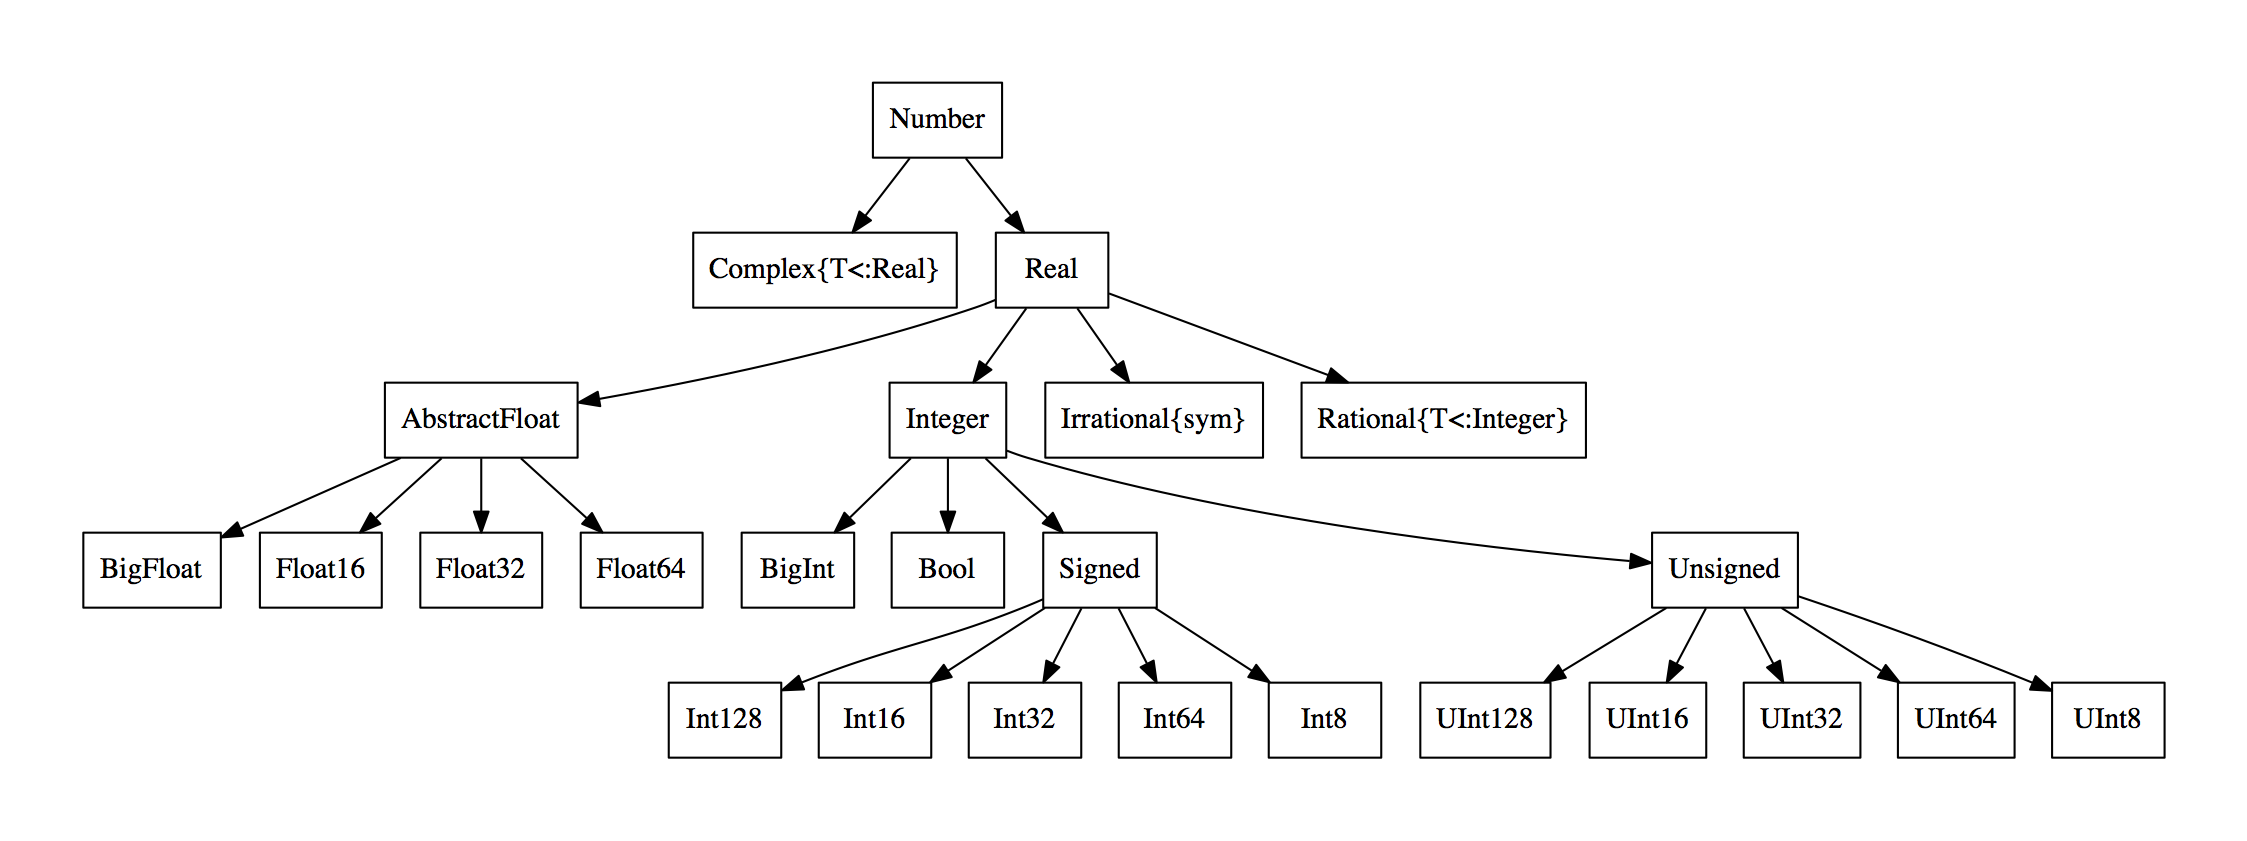
\includegraphics[width=1.0\textwidth]{types}
  \end{figure}
\end{frame}

\begin{frame}[fragile]
	\frametitle{Modules}
  \begin{tiny}
  \begin{minted}{julia}
module MyModule
using Lib

using BigLib: thing1, thing2

import Base.show

importall OtherLib

export MyType, foo

type MyType
    x
end

bar(x) = 2x
foo(a::MyType) = bar(a.x) + 1

show(io::IO, a::MyType) = print(io, "MyType $(a.x)")
end
  \end{minted}
  \end{tiny}
\end{frame}

\begin{frame}[fragile]
	\frametitle{Modules}
  \begin{tiny}
  \begin{minted}{julia}
module Normal
include("mycode.jl")
end

module Testing
include("safe_operators.jl")
include("mycode.jl")
end
  \end{minted}
  \end{tiny}
\end{frame}

\begin{frame}[fragile]
	\frametitle{Testing}
  \begin{tiny}
  \begin{minted}{julia}
julia> using Base.Test

julia> foo(x) = length(x)^2
foo (generic function with 1 method)

julia> @test foo("bar") == 9
Test Passed
  Expression: foo("bar") == 9
   Evaluated: 9 == 9

julia> @testset "Foo Tests" begin
           @test foo("a")   == 1
           @test foo("ab")  == 4
           @test foo("abc") == 9
       end
Test Summary: | Pass  Total
Foo Tests     |    3      3
  \end{minted}
  \end{tiny}
\end{frame}

\begin{frame}[fragile]
	\frametitle{The real world}
  \begin{tiny}
  \begin{minted}{julia}
using DifferentialEquations

srand(100)

prob = prob_sde_additive
sol =solve(prob,dt=1/2^(3))
@test typeof(sol.alg) == SRIW1

sol =solve(prob,dt=1/2^(3),alg_hints=[:additive])
@test typeof(sol.alg) == SRA1
  \end{minted}
  \end{tiny}
  \vspace{5.0mm}
   https://github.com/JuliaDiffEq/DifferentialEquations.jl
\end{frame}
